\documentclass[17pt]{extarticle}
\usepackage{tikz}
\usetikzlibrary{
   shadings,
   shadows,
}

\begin{document}
\noindent
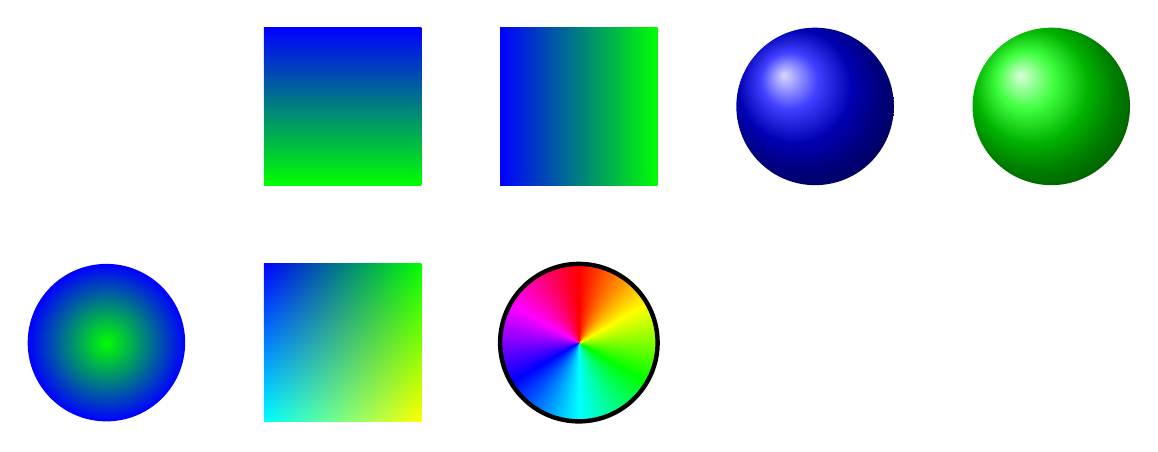
\begin{tikzpicture}
\shade [top color = blue, bottom color = green]
      (3,0) rectangle (5,2);
\shade [left color = blue, right color = green]
       (6,0) rectangle (8,2);
\shade [shading = ball] (10,1) circle [radius=1];
\shade [ball color = green] (13,1) circle [radius=1];
\shade [inner color = green, outer color = blue]
       (1,-2) circle [radius = 1];
\shade [
      upper left = blue,
      upper right = green,
      lower right = yellow,
      lower left = cyan,
   ] (3,-3) rectangle (5,-1);
   
\shadedraw [ultra thick, shading = color wheel]
      (7,-2) circle [radius = 1];
\end{tikzpicture}

\end{document}